\section{Implementation}
\label{sec:implementation}
In this section, we discuss the technical implementation of Jorvik which underpins the process of our approach discussed in the previous section. 


\begin{figure}[ht!]
	\centering
	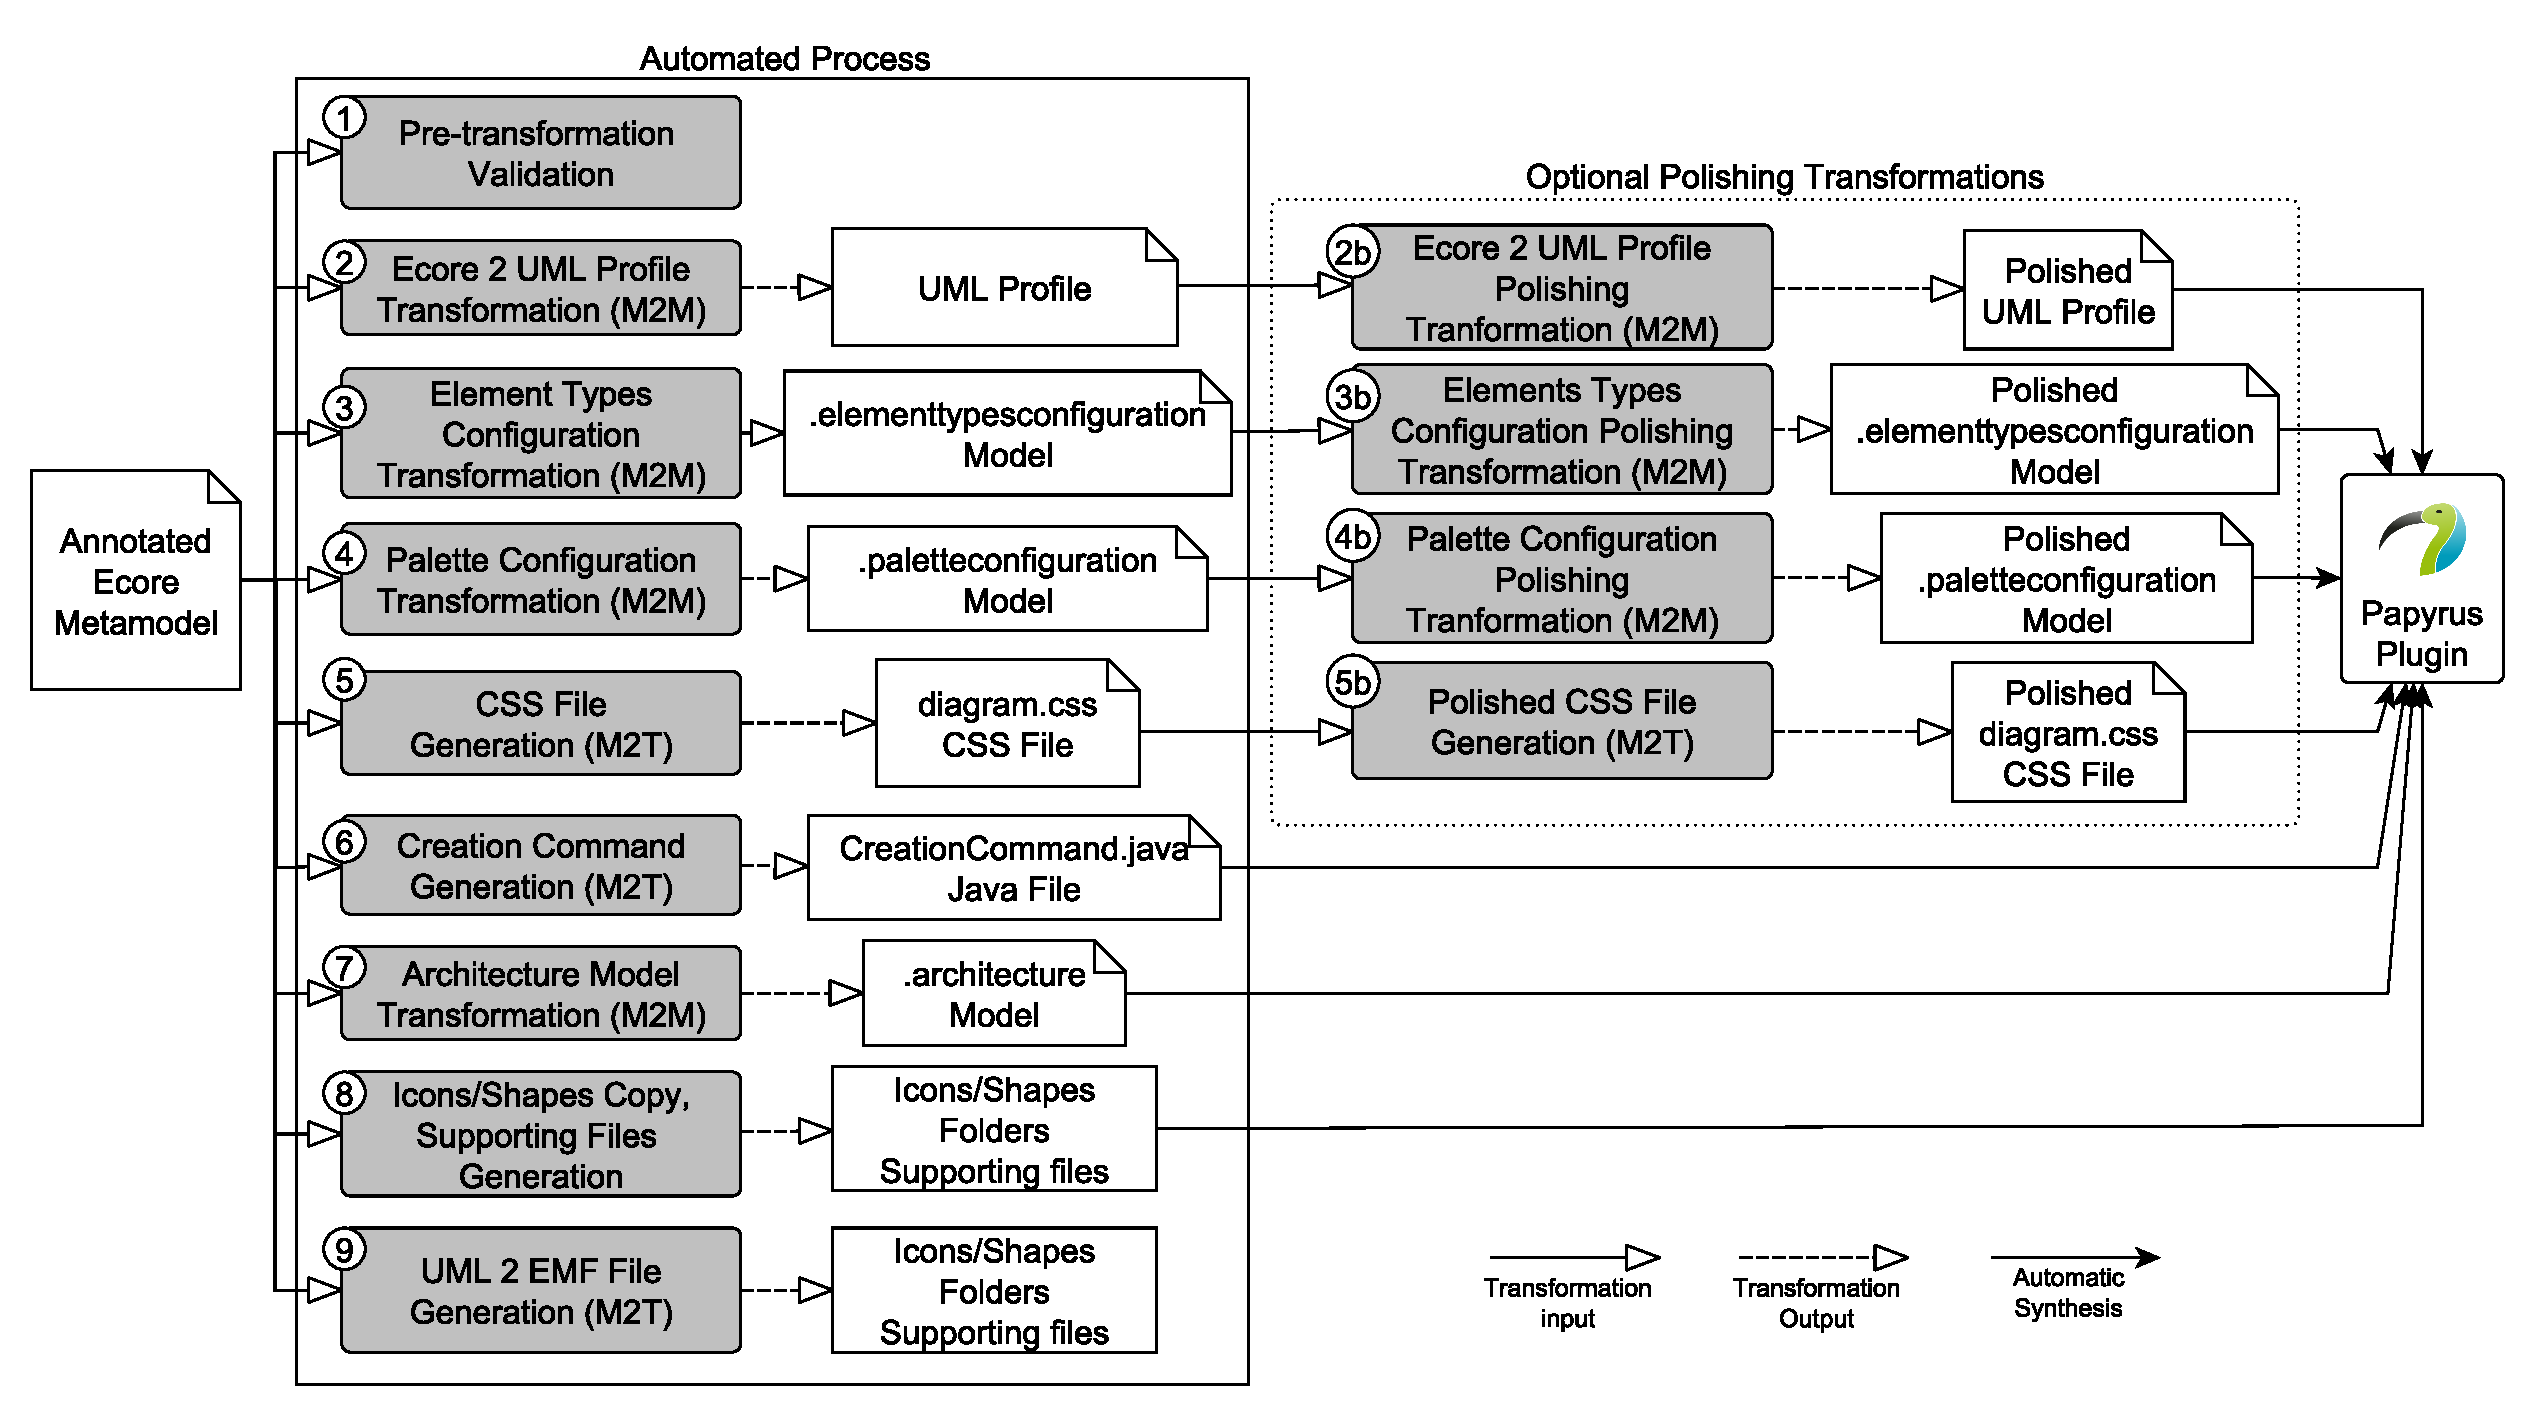
\includegraphics[width=1\textwidth]{diagrams/transformationWorkflow.pdf}
	\caption[]{An overview of the transformation workflow}
	\label{fig:transformationWorkflow}
	%	\vspace*{-3mm}
\end{figure}

Figure~\ref{fig:transformationWorkflow} shows workflow of \textit{Jorvik}. 
Each step in the workflow is identified by a number (\#1 -- \#9 in Figure~\ref{fig:transformationWorkflow}) for easier reference. 
Before generating all the artefacts, a pre-transformation validation script (\#1 in Figure~\ref{fig:transformationWorkflow}) is executed to verify the correctness of the annotations, and provide useful feedback to the users if there is anything wrong. 
Moreover, supporting files needed for the creation of the Papyrus Plug-in are also generated while icons and shapes are placed next to the annotated metamodel (\#8 in Figure~\ref{fig:transformationWorkflow}). 
As the transformations consist of about 1000 lines of code we will describe them omitting low level technical details\footnote{Full implementations and instructions are available at \url{https://github.com/wrwei/Jorvik}}. 


\subsection{Pre-transformation Validation (\#1)}
To check the correctness of the annotated Ecore metamodel, a model validation program is firstly executed against the metamodel.
The program is written using EVL and consists of several rules that check if the annotated Ecore elements have all the necessary information (e.g., a UML base class) and if the values provided are correct (e.g., font size for labels is a positive integer). 
Listing~\ref{lst:evlRulesBold} presents an example of a rule written in EVL which checks if the value provided for the ``bold'' details in a @Node annotation is correct (i.e., true or false). More specifically, in lines 2--3 a guard is applied to check that the rule is only applied to elements that have the @Node annotation attached to them (line 2) while it tests the rule only on those annotations that have the ``bold'' detail defined (line 3). 
In lines 4--6, the condition to check is provided, which is that the value of the ``bold'' detail is either \textit{true} or \textit{false}. 
Finally, in lines 7--8 a message is displayed to the users in case the rule is violated providing information regarding the acceptable values and the name of the element(s) that violated this rule.

\lstinputlisting[
caption={Example rule that checks that the values provided to the ``bold'' styling detail for @Node annotations is correct.},
label={lst:evlRulesBold},
captionpos=b, 
language=EVL, 
tabsize=2, 
numbers=left, 
numbersep=5pt, 
numberstyle=\tiny, 
breaklines=6true]{evlRulesBold.evl}

\begin{table}[ht!]
	\begin{tabular}{|l|L{5cm}|L{5cm}|}
		\hline
		\textbf{\#} & \textbf{Rule Description} & \textbf{Condition Checked} \\ \hline
		1 & There is exactly one Diagram annotation & The number of the @Diagram annotations is 1 \\ \hline
		2 & Diagram annotation has a name detail & The name detail is defined \\ \hline
		3 & Diagram annotation has acceptable details provided & There are no other details provided rather than name and/or icon \\ \hline
		4 & Node/Edge annotations have base class set & Any string is provided\\ \hline
		5 & Edge annotations of EClasses have source/target defined & The source/target details are defined \\ \hline
		6 & An acceptable lineStyle value for Edge annotations is provided & The value is dashed, solid, dotted, hidden or double\\ \hline
		7 & An acceptable bold value for Node/Edge annotations is provided & The value is either true or false\\ \hline
		8 & An acceptable fontHeight value for Node/Edge annotations is provided & The value is a positive integer\\ \hline
		9 & Node annotations have acceptable details provided & There are no other details provided rather than base, fontHeight and/or bold \\ \hline
		10 & Edge annotations have acceptable details provided & There are no other details provided rather than base, source, target, fontHeight, bold, and/or lineStyle\\ \hline
	\end{tabular}
	\caption{The list of the rules checked for the annotated Ecore metamodel.}
	\label{tab:evlRules}
\end{table}

Table~\ref{tab:evlRules} enumerates all the rules included in the pre-transformation validation step along with their descriptions and the conditions that are checked. 
%The implementation of the rules in EVL can be found in the Jorvikwebpage\footnote{\url{https://github.com/wrwei/Jorvik}}. 


\subsection{EMF to UML Profile Generation (\#2)}
\label{sec:profileGeneration}
The EMF to UML Profile Generation executes a model-to-model transformation written in ETL. 
The source model of this transformation is the annotated Ecore metamodel (e.g.,  Listing~\ref{lst:annotatedSdplEmfatic}) and the target model is a UML profile model.
This transformation consists of two main rules, one that creates a Stereotype for each EClass element of the metamodel and a second that creates a \textit{Stereotype} for each EReference annotated as @Edge:

\begin{itemize}
	\item[--] \textbf{rule eclass2stereotype:} This transformation rule transforms each EClass element in the annotated Ecore metamodel to an element of type stereotype in the target UML model. 
	All attributes of each EClass are also transformed across to the created stereotype. 
	\item[--] \textbf{rule reference2stereotype:} This rule creates a new stereotype with the same name in the UML profile model for each of the EReferences that are annotated as @Edge in the Ecore metamodel. 
	No attributes are added to the stereotype as EReferences do not support attributes in Ecore\footnote{It is the users' responsibilities to make sure that they handle name collisions for EReferences themselves (for that EClasses may have EReferences with the same name).}.
\end{itemize}

When all stereotypes are created, a number of post-transformation operations are executed to 1) create the generalisation relationships between the stereotypes, 2) add the references/containment relationships between the stereotypes, 3) create the extension with the UML base meta-element and 4) generate and add the needed OCL constraints for each edge: 

\begin{enumerate}[label=\arabic*)]
	\item For each superclass of an EClass in the metamodel we create a \textit{Generalisation} UML element. 
	The generalisation element is added to the stereotype created for this specific EClass and refers via the \textit{generalization} reference to the stereotype that was created for the superclass.
	\item For each reference (ref or val) in the metamodel a new \textit{Property} UML element is created and added to the stereotype that represents the EClass. 
	A new \textit{Association} UML element is also created and added to the stereotype. The name and the multiplicities are also set.
	\item By default the stereotypes extend the \textit{Class} base element unless a different value is passed in the \textit{base} property of the @Node/@Edge annotation. 
	In this post-transformation operation the necessary \textit{Import Metaclass} element and \textit{Extension} reference are created and attached to the stereotype.
	\item In the last operation, the OCL constraints are created for each stereotype that will be represented as an edge on the diagram. 
	Two \textit{Constraint} and two \textit{OpaqueExpression} elements are created for each edge stereotype that check the two necessary constraints. 
	The OCL constraints are explained in details in the section that follows.
\end{enumerate}

\subsection{OCL Constraints}
\label{sec:constraints}

To illustrate the OCL constraints, we provide a partial view of the SDPL UML profile in Figure \ref{fig:sample_profile}\footnote{The attributes of the stereotypes are omitted for simplicity.}.

\begin{figure}[ht!]
	\centering
	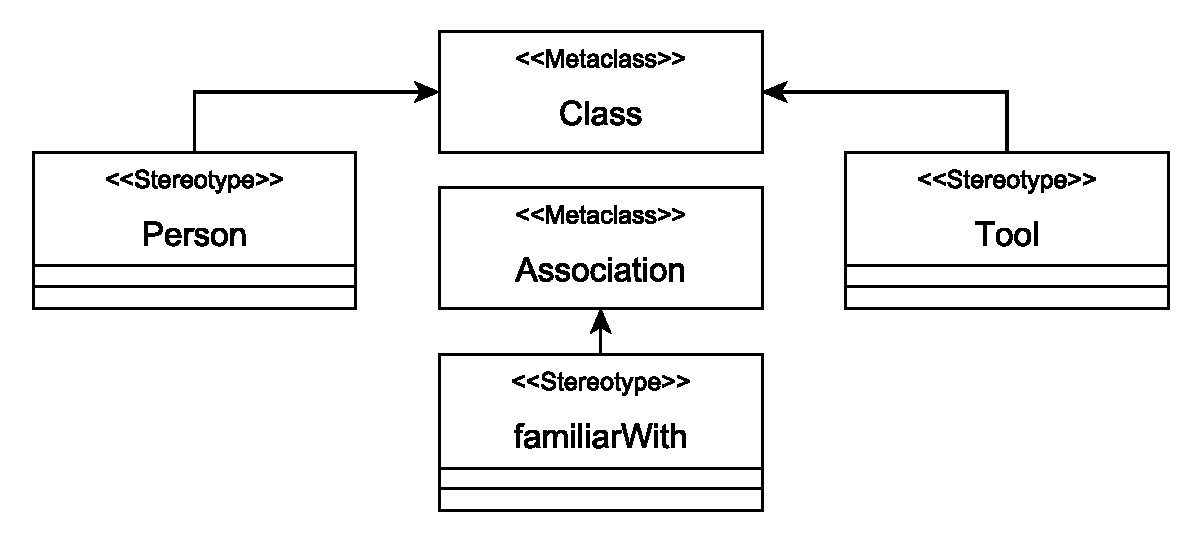
\includegraphics[width=1\textwidth]{diagrams/example_profile}
	\caption[]{Example UML profile for SDPL showing Person, Tool and the familiarWith association}
	\label{fig:sample_profile}
\end{figure}

In Figure \ref{fig:sample_profile}, there are three \textit{Stereotype}s. ``Person" and ``Tool" extend meta-element UML::Class, and they correspond to classes ``Person" and ``Tool" in the metamodel shown in Listing \ref{lst:annotatedSdplEmfatic}. 
Stereotype ``familiarWith", which extends meta-element UML::Association, corresponds to the reference``familiarWith" in the ``Person" class in Listing \ref{lst:annotatedSdplEmfatic}.

In Figure~\ref{fig:sdplEditor}, the ``familiarWith" association is used to connect ``Person Alice" with ``Tool StarUML". 
However, Papyrus by default, allows the ``familiarWith: stereotype to be applied to any \emph{Association}, and not strictly to \emph{Associations} which connect ``Person" and ``Tool" stereotyped elements. 
Therefore, constraints are needed to check (at least) two aspects:

\begin{itemize}
	\item \textbf{End Types}: one of the elements a ``familiarWith" association connects to, has the ``Person" steretotype applied to it while the other has the ``Tool" stereotypes applied to it;
	\item \textbf{Navigability}: the ``familiarWith" association starts from an element stereotyped as ``Person" and points to an element stereotyped as ``Tool".
\end{itemize}

\subsubsection{End Types}
Listing \ref{lst:endTypes} shows the OCL code for the \emph{End Types} constraint. 
Line 1 accesses the types (instances of UML::Class that have stereotypes defined in the profile applied to them) that ``familiarWith" connects. 
Lines 3 and 4 check if the types that ``familiarWith" connects are of type that either has stereotype ``Person" or ``Tool". 
In this way, if a ``familiarWith" association connects two types that are not ``Person" or a ``Tool", the constraint fails.

\lstinputlisting[
	caption={The End Types constraint in OCL},
	label={lst:endTypes}, 
	captionpos=b, 
	language=OCL, 
	tabsize=2, 
	numbers=left, 
	numbersep=5pt, 
	numberstyle=\tiny, 
	breaklines=true, 
	escapeinside={(*}{*)}]{endtypes.txt}

\subsubsection{Navigability}
Listing \ref{lst:navigability} shows the OCL code for the \emph{Navigability} constraint. 
In this case, we are interested in checking the \emph{isNavigable} property of each end. 
Thus, in lines 2 and 3, we obtain the member ends that ``familiarWith" connects with. 
If these ends are obtained successfully (line 4), we check that the \emph{personEnd} (connecting element stereotyped as ``Person") is not navigable (line 5) and the \emph{toolEnd} (connecting element stereotyped as ``Tool") is navigable (line 6). 
Therefore, we are checking that a ``familiarWith" association can only go from ``Person" to ``Tool" and not the other way around. 
We need to highlight, that currently, opposite references are not supported; plans for future work are outlined in Section~\ref{sec:future}.

\begin{figure}[h]
	\lstinputlisting[caption={The Navigability constraint in 
		OCL},label={lst:navigability}, captionpos=b, language=OCL, tabsize=2, 
	numbers=left, numbersep=5pt, numberstyle=\tiny, breaklines=true, 
	escapeinside={(*}{*)}]{navigability.txt}
%	\vspace*{-5mm}
\end{figure}

With these two constraints implemented, we are able to automatically generate OCL constraints for stereotypes that extend UML::Association. 
We use the \emph{End Types} and \emph{Navigability} constraints as templates with dynamic sections (where the specific stereotype names are inserted dynamically, e.g., ``Person" and ``Tool"). 
So far we have only explored constraints for stereotypes that extend UML::Association. 
The constraint templates for stereotypes that extend other UML relationships need to be developed separately as the means to access source/target elements of the relationship are different.

\subsection{Element Types  Configuration Transformation(\#3)}
\label{sec:elementTypes}
Apart from the UML profile, Papyrus graphical editors require an Element Types Configuration model, which associates the \textit{Stereotype}s defined in the UML profile with their abstract syntax (the meta-elements in UML they extend) and their concrete syntax (the graphical notations of the meta-elements in UML they extend). 

This transformation is responsible for creating an Element Types Configuration model (of extension .elementtypesconfiguration) that contains type specialisation information for the stereotypes in the UML profile. 
%Since our previous work \cite{zolotas2018towards}, the \textit{ElementTypesConfiguration} metamodel for Papyrus has changed. 
%As a result, we have to re-implement this transformation. 
For each element of type \textit{Stereotype}, two \textit{SpecializationTypeConfiguration}s are created, one links the stereotype to its UML meta-element, another links the stereotype to the concrete syntax of its UML meta-element.
For example, a stereotype that extends UML::Class needs to specialise the UML::Class \textit{MetamodelTypeConfiguration} defined in the UML Element Types Configuration model; and it needs to specialise the Class Shape \textit{SpecializationTypeConfiguration} defined in the UML Diagram Element Types Configuration model\footnote{Both models reside in the Papyrus Plug-in \textit{org.eclipse.papyrus.uml.service.types}}. 
In addition to \textit{SpecializationTypeConfiguration}s, for each \textit{Stereotype} element an \textit{ApplyStereotypeAdviceConfiguration} needs to be created, which associates the \textit{SpecializationTypeConfiguration} to the actual stereotype in the UML profile.

%The transformed Element Types Configuration model is a crucial part to Papyrus graphical editor creation, it is used in conjunction with other models/artefacts and it drives the creation of model elements in the editor.

\subsection{Palette Configuration Transformation (\#4)}
\label{sec:paletteGeneration}
This transformation is responsible for creating a Palette Configuration model (of extension .paletteconfiguration) that configures the contents of the custom palette for the diagram in Papyrus. 
The model conforms to the \textit{PaletteConfiguration} metamodel that ships with Papyrus.
%which also changed since our previous work. 
The transformation creates a new \textit{PaletteConfiguration} element and adds two new \textit{DrawerConfiguration} elements that represent two different tool compartments in our palette (i.e., one for the tools that create nodes and one for those creating edges). 
For each element in the Ecore metamodel annotated as @Node/@Edge a new \textit{ToolConfiguration} element is created and added to the nodes/edges drawer respectively. 
The kind of \textit{ToolConfiguration} are decided based on the @Node/@Edge annotation. For nodes, the kind is \textit{CreationTool} while for edges, the kind is \textit{ConnectionTool}.
An \textit{IconDescriptor} element is also created and added to the \textit{ToolConfiguration} pointing to the path of the icon for that tool (this is the path passed as argument to the \textit{icon} property of the @Node/@Edge annotation).
Finally, each \textit{ToolConfiguration}, needs to refer to the element types they conform to, which are defined in the Element Types Configuration model transformed in Step \#3. 
In this way, when an element is created in the diagram using the palette, behind the scene, Papyrus is able to locate the \textit{Stereotype} element and determine the UML syntax it specialises.

\subsection{CSS File Generation (\#5)}
\label{sec:cssGeneration}
As stated above, the look and feel of diagram elements in Papyrus can be customised using CSS. 
In this transformation we generate our default CSS style rules that define the appearance of nodes and edges in diagrams. 
Each node on a diagram has a set of compartments where the attributes, shapes, etc. appear. 
Initially, for all nodes that will appear on the diagram, we create a CSS rule to hide all their compartments and another rule to enable the compartment that holds the shape. 
The latter rule also hides the default shape inherited from the meta-element that the stereotype extends. 
Then, for each stereotype that appears as a node, a CSS rule is generated to place the SVG figure in the shape compartment. 
For elements of type \textit{Stereotype}, the assignment of the SVG shapes to the stereotypes is achieved by assigning the path of the SVG file to the \textit{svgFile} property available in CSS. 
Finally, we generate the CSS rules for each edge, e.g., if a \emph{lineStyle} parameter is set, then the \textit{lineStyle} property for that stereotype is set to the value of the lineStyle parameter (e.g., ``solid'', ``dashed'', etc.).

\subsection{Creation Command Generation (\#6)}
\label{sec:creationCommand}
In order for Papyrus to create a diagram, it requires the initialisation of the diagram.
The Creation Command is a Java class which is responsible for initialising Papyrus diagrams. 
The Creation Command class is needed since Papyrus 3.0+.
The rationale for the creation command is that it creates a UML model from the UMLFactory as the root element of the diagram.
The minimal requirement for diagram initialisations are:
\begin{itemize}
	\item UML primitive types: the primitive types need to be imported to the diagram in order for the users to reference to them;
	\item UML profiles: the standard UML profile and the user defined UML profile need to be applied in order to initialise the diagram.
\end{itemize}

In order to apply the user defined UML profiles, they need to use the pathmap defined in their plug-ins, which is explained in \#8.
The Java class is generated using a model-to-text transformation written in EGL.
%with the source model the annotated Ecore metamodel and the output text the CreationCommand.java class.

\subsection{Architecture Model Generation (\#7)}
\label{sec:architectureModel}
Papyrus adopted the notion of an Architecture model in order to describe the architecture of the graphical editors since Papyrus 3.0+.
This transformation synthesises an Architecture model using a model creation program written in the Epsilon Object Language (EOL) \cite{kolovos2006epsilon}. 
The program needs 1) the annotated Ecore metamodel for the DSL, 2) the Element Types Configuration model, 3) the Palette Configuration model, 4) the UML metamodel, 5) the Creation Command Java class and 6) the CSS custom style sheet as inputs. 
In particular, in the Architecture model, the generation program creates:
\begin{itemize}
	\item An \textit{ArchitectureDomain} which represents the domain of the DSL;
	\item A number of \textit{Concern}s to describe the concerns of the domain;
	\item A number of \textit{Stakeholder}s involved in the domain;
	\item An \textit{ArchitectureDescriptionLanguage} to describe the architecture, which consists of a number of \textit{Viewpoint}s, a number of \textit{PapyrusDiagram}s. 
	The Element Types Configuration and the Creation Command class are needed in the \textit{ArchitectureDescriptionLanguage}. 
	The Palette Configuration model and the CSS sheets are needed in \textit{PapyrusDiagram}s.
\end{itemize}

The Architecture model then needs to be registered and acts as the entry point to all the models/files for a Papyrus editor, which is done in Step \#9.

\subsection{Icons, Shapes and Supporting Files (\#8)}
\label{sec:supportingFiles}
\textit{Jorvik} supports the generation of the UML profile and the infrastructure for the Papyrus diagram in either a new Eclipse plug-in project or in the same plug-in project where the annotated Ecore metamodel resides. 
In both scenarios, the ``MANIFEST.MF'', the ``build.properties'' and the ``plugin.xml'' files are created (or overridden respectively). 
%The first includes the list of all the required bundles while the second points the project to the locations of the ``MANIFEST.MF'' and ``plugin.xml'' files. 
The ``MANIFEST.MF'' file includes a list of all required bundles/plug-ins.
The ``build .properties'' file guides the build process of the Eclipse plug-in.
The ``plugin.xml'' file includes all the necessary extensions for Papyrus to be able to register the UML profile and create the diagrams (e.g., extensions that point to the Architecture model). 
For the creation of a Papyrus editor, in the ``plugin.xml'', three extension points need to be implemented:
\begin{itemize}
	\item \textit{org.eclipse.emf.ecore.uri\_mapping}, in which the users create a mapping between the path of the folder that hold their UML profile, and a PATHMAP, which they can reference in the files/models they create;
	\item \textit{org.eclipse.papyrus.uml.extensionpoints.UMLProfile}, which points to the location of the UML profile that the users define;
	\item \textit{org.eclipse.papyrus.infra.architecture.models}, which points to the location of the Architecture model that the users define in Step \#7.
\end{itemize}

For the scenario where the Papyrus plug-in is created as a new project, the shapes (SVG files) and the icons (PNG files) are copied to the newly created Plug-in project. 
For the scenario where the UML profile and editor are generated in the same project in which the Ecore source file resides, the shapes and icons files do not need to be copied as they already exist.

Finally, two files that only consist of the XML and the XMI header (namely ``*.profile.di'' and ``*.profile.notation'') are generated. 
These files are necessary for Papyrus to construct the UML profile model\footnote{The diagram layout information requires coordinates related information in the diagram, therefore it is not related to this work}. 

\subsection{UML to EMF Transformation Generation (\#9)}
\label{sec:uml2emf}
\lstinputlisting[
caption={Example of an auto-generated ETL rule that transforms \\elements stereotyped as ``Person'' in the UML model to elements of \\type ``Person'' in an EMF model.},
label={lst:etlGeneratedRule},
captionpos=b, 
language=ETL, 
tabsize=2, 
numbers=left, 
numbersep=5pt, 
numberstyle=\tiny, 
breaklines=true]{etlExample.etl}

This M2T transformation generates the ETL file that can be used to transform the UML models created in Papyrus and conform to the UML Profile generated by our approach, back to EMF models that conform to the source Ecore metamodel given as input to the approach. 
One rule is generated for each of the stereotypes that transforms them back to the appropriate type of the Ecore metamodel. 
Each stereotype has the same attributes and references as the original EClass, therefore, this EGL script also generates the statements in each rule that populate the attributes and the references of the newly created instance of each EClass with the equivalent values of the UML model. 
An example of an auto-generated rule is shown in Listing~\ref{lst:etlGeneratedRule}. 
This rule transforms elements stereotyped as ``Person'' in the UML model to elements of type ``Person'' in an EMF model which conforms to the Ecore metamodel presented in Listing~\ref{lst:annotatedSdplEmfatic}.


%Epsilon Transformation Language (ETL) \cite{} is a hybrid model-to-model transformation languages which provides both a declarative rule-based execution scheme and imperative features for handling complex transformation scenarios. In Listing~\ref{lst:etlGeneratedRule}, rule \emph{PersonUML2PersonEMF} is responsible to transform a \emph{Person} in the UML model to a \emph{Person} in the EMF model. 

ETL provides the $::=$ operator for rule resolution. 
The ETL engine keeps transformation traces which links source elements to target elements of the transformation. 
When $::=$ is used, the ETL execution engine inspects the established transformation traces and invokes the applicable rules (if necessary) to calculate the counterparts of the source elements contained in the collection. 

%If \emph{equivalents()} is applied to a single element, it returns a collection which contains the counterpart(s) of the element in the target model. If \emph{equivalents()} is applied to a collection of elements, it returns a collection of collection (each collection in the result contains the counterparts of the element in the target model). 

In our example (line 6 in Listing \ref{lst:etlGeneratedRule}), the expression ``s.familiarWith'' returns a collection of \emph{UMLProcess!Tool}s (denoted by $ct$). By using ``::='', the ETL engine will look for the rules that transform \emph{UMLProcess!Tool} to \emph{EMFProcess!Tool} and invoke the rules if 
necessary (if the source elements have not been transformed, as shown in the transformation trace) and put the transformed elements into sub-collections 
(denoted by $sc$). 
After the ETL engine goes through all the elements in $ct$, the sub-collections $sc$s are returned (flattened to a single collection if more than one) and are added to ``t.familiarWith''.



\subsection{Polishing Transformations (\#2b - \#5b)} 
\label{sec:transformationPatches}

\begin{table}[h]
	\caption{Polishing Transformations File Names}
	\centering
	\setlength{\tabcolsep}{3.5pt} 
	\begin{tabular}{|c|c|}
		\cline{1-2}
		\textbf{Transformation ID}  & \textbf{Required File Name}\\ \hline
		\textbf{\#2} & emf2umlProfile.etl\\ \hline
		\textbf{\#3} & elementTypesConfigurationsM2M.etl\\ \hline
		\textbf{\#4} & paletteConfigurationM2M.etl\\ \hline
		\textbf{\#5} & cssFileGeneration.egl\\ \hline
		\cline{1-2}
	\end{tabular}
	\label{tab:polishingTransformationsNames}
\end{table}

For transformations \#2- \#5, users are able to define polishing transformations that complement those included in our implementation. 
After each built-in transformation is executed, the workflow looks to find a transformation with the same file name next to the Ecore metamodel. 
If a file with the same name exists, it is executed against the Ecore metamodel and targets the already created output model of the original transformation. 
The execution of the polishing transformation is set \textit{not} to overwrite the target model but to refine it instead.
Table~\ref{tab:polishingTransformationsNames} shows the names that each polishing transformation is expected to have.

\subsection{Adding support for nested relations}
In EMF, a reference between two classes can be flagged as a containment relation, which is consistent with the \emph{containment} definition of UML associations (with exception of the deletion cascade mechanism).
These types of relations, when presented visually, can benefit from showing the contained elements shapes inside the shape of the container, as opposed to the line/arrow presentation.
For example, if a \texttt{package} is represented with an empty rectangle, classes contained in the package would appear inside this rectangle.

Ideally, a custom profile editor should allow this containment relations to be represented as visual containment too.
Papyrus does allow providing custom shapes for elements, so we explored the feasibility of supporting visual containments too.
However, the current structure of the Papyrus visual editor does not allow this functionality.
Currently, the \emph{shape} concept at the editor level provides separate graphical sections for the custom shape and the contained elements.
These two sections are presented visually one after the other.
Hence, with the current Papyrus implementation it is not possible to have nested elements inside a custom shape.

